\documentclass{article}
\usepackage[utf8]{inputenc}
\usepackage[T1]{fontenc}
\usepackage[english]{babel}
\setlength{\parindent}{0pt}
\usepackage{hyperref}
\hypersetup{
    colorlinks=true,
    linkcolor=blue,
    filecolor=magenta,      
    urlcolor=cyan}
\usepackage{graphicx}
\graphicspath{ {./pic/} }
\usepackage{multicol}
\usepackage{lscape}

\usepackage{fourier,amssymb,microtype,amsmath,gensymb}
\newcommand{\R}{\mathbb{R}}
\usepackage{mdframed,caption,xcolor}
\usepackage{tikz,tkz-euclide}

\title{Seminar 12. Auctions and previous exam problems}
\author{Xiaoguang Ling \\  \href{xiaoguang.ling@econ.uio.no}{xiaoguang.ling@econ.uio.no}}
\date{\today}

\begin{document}

\maketitle

%%%%%%%%%%%%%%%%%%%%%%%%%%%%%%%%%%%%%%%%%%%%%%%%%%%%%%%%%%%%%%%%%%%%%%%%%%%%%%%%%%%%%%%%%%%%%%
\section{Jehle \& Reny pp.484, exercise 9.2}

Show in two ways that the symmetric equilibrium bidding strategy of a first-price auction with $N$
symmetric bidders each with values distributed according to $F$, can be written as


$$\hat{b}(v) = v -\int_{0}^{v} \left(\frac{F(x)}{F(v)}\right)^{N-1} dx$$

For the first way, use our solution from the text and apply integration by parts. For the second
way, use the fact that $F^{N-1}(r)(v - \hat{b}(r))$ is maximised in r when $r = v$ and then apply the envelope
theorem to conclude that $d(F^{N-1}(v)(v - \hat{b}(v))/dv = F^{N-1}(v)$; now integrate both sides from $0$ to $v$.

\bigskip

See lecture notes for the third lecture on the economics of information (on ``Auctions and the revenue equivalence theorem''), pages 17 and 19.


\section{Jehle \& Reny pp.484, exercise 9.1 - Show that the bidding strategy in (9.5) is strictly increasing.}

By exercise 9.1, the bid function can be written as:$$\hat{b}(v_i) = v_i - \frac{\int_0^{v_i}[F(x)]^{N-1} dx}{[F(v_i)]^{N-1}} \, .$$

Then:

\begin{align*}
  \frac{d}{dv_i}\left( \hat{b}(v_i) \right) &= \frac{d}{dv_i}\left( v_i - \frac{\int_0^{v_i}[F(x)]^{N-1} dx}{[F(v_i)]^{N-1}} \right) \\
  &= 1 - \frac{[F(v_i)]^{N-1}}{[F(v_i)]^{N-1}} + \frac{\int_0^{v_i}[F(x)]^{N-1} dx }{[F(v_i)]^{2N-2}} \cdot \frac{d}{dv_i}\left( [F(v_i)]^{N-1} \right) \\
  &= \frac{\int_0^{v_i}[F(x)]^{N-1} dx }{[F(v_i)]^{2N-2}} \cdot (N-1) [F(v_i)]^{N-2} f(v_i) > 0 \, .
\end{align*}

\bigskip

\section{Jehle \& Reny pp.485, exercise 9.3}

This exercise will guide you through the proof that the bidding function in (9.5) is in fact a symmetric
equilibrium of the first-price auction.

\subsection*{(a)} Recall from (9.2) that
$$\frac{du(r,v)}{dr}=(N-1)F^{N-2}(r)f(r)(v-\hat{b}(r))-F^{N-1}(r)\hat{b'}(r).$$
Using (9.3), show that


\begin{align*}
\frac{du(r,v)}{dr}&=(N-1)F^{N-2}(r)f(r)(v-\hat{b}(r))-(N-1)F^{N-2}(r)f(r)(r-\hat{b'}(r)) \\
&= (N-1)F^{N-2}(r)f(r)(v-r)
\end{align*}

\subsection*{(b)}Use the result in part (a) to conclude that $du(r, v)/dr$ is positive when $r < v$ and negative when
$r > v$, so that $u(r, v)$ is maximised when $r = v$.
\bigskip
See https://www.uio.no/studier/emner/sv/oekonomi/ECON4240/previous-exams/ECON4240-2005V-SENSORVEILEDNING.pdf as well as a solution sketch available in Canvas

\section{Problems 2  of the exam in ECON4240, Spring 2005}


Consider a strategic situation between an employer (E) and a worker (W). E can either accept
(A) or reject (R) W. W can either become skilled (S) through education, or remain unskilled
(U). W can be of two types; either he is inherently high ability (H) or he is inherently low
ability (L). The players' payoffs depending on their actions and W's type is shown below.

{\centering
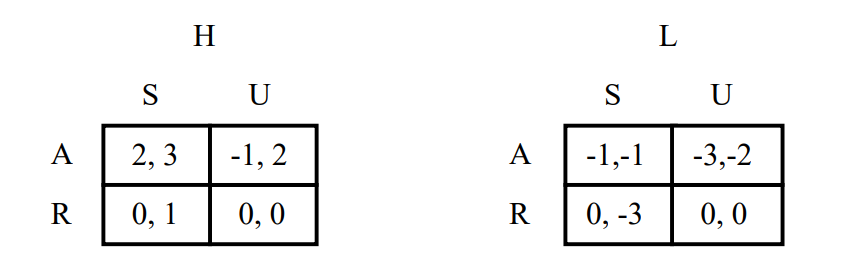
\includegraphics[width=0.8\textwidth]{12.q2}
\vspace{2mm}}


\subsection*{a)} For each of these games, determine the set of (pure) rationalizable strategies for each
player, and the set of pure-strategy Nash equilibria.
\subsection*{b)} Assume next that only W knows his own type, while player E thinks that the two types
of W are equally likely. Model this situation in an ex ante perspective by specifying
the Bayesian normal form.
\subsection*{c)} For the Bayesian normal form found in part (b), determine the set of (pure)
rationalizable strategies for each player, and the set of pure-strategy and/or mixedstrategy Nash equilibria.

\section{Problems 3  of the exam in ECON4240, Spring 2005}

Problem 3 (20 \%)
Consider again the strategic situation between an employer (E) and a worker (W) described in
Problem 2. Assume (as in parts b and c) of Problem 2) that only W knows his own type, while
player E thinks that the two types of W are equally likely.
\subsection*{a) (Screening)} Assume now that E acts before W, and that E's choice of A or R can be
observed by W before he makes his choice of S or U. Show that there is a unique
subgame perfect Nash equilibrium.
\subsection*{b) (Signaling)} Assume now that W acts before E, and that W's choice of S or U can be
observed by E before she makes her choice of A or R. Show that there is a unique
perfect Bayesian equilibrium.


\end{document}
